\section{標準形式トレースログ}

本節では,標準形式トレースログを定義するために行ったトレースログの抽象化と,標準形式トレースログの定義について述べる.

\subsection{トレースログの抽象化}

標準形式トレースログを提案するにあたり,トレースログの抽象化を行った.

はじめに,トレースログを,時系列にイベントを記録したものと考えた.
次に,イベントとはイベント発生源の属性の変化,イベント発生源の振る舞いと考えた.
ここで,イベント発生源をリソースと呼称し,固有の識別子をもつものとする.
つまり,リソースとは,イベントの発生源であり,名前を持ち,固有の属性をもつものと考えることができる.

リソースは型により属性,振る舞いを特徴付けられる.
ここでリソースの型をリソースタイプと呼称する.

属性は,リソースが固有にもつ文字列,数値,真偽値で表されるスカラーデータとし,振る舞いはリソースの行為であるとする.

リソースタイプとリソースの関係は,オブジェクト指向におけるクラスとオブジェクトの関係に類似しており,属性と振る舞いはメンバ変数とメソッドに類似している.
ただし,振る舞いはリソースのなんらかの行為を表現しており,メソッドの,メンバ変数を操作するための関数や手続きを表す概念とは異なる.

主に,振る舞いは,属性の変化を伴わないイベントを表現するために用いる.
振る舞いは任意の数のスカラーデータを引数として受け取ることができ,これは,図形描画の際の条件,あるいは描画材料として用いられることを想定している.

図\ref{fig:resourceTypeSample}と図\ref{fig:resourceSample}に,リソースタイプとリソースを図で表現した例を示す.
さらに,図\ref{fig:resourceTypeSampleByTask}に,RTOS(Real-time operating system)におけるタスクの概念をリソースタイプとして表現した例を,図\ref{fig:resourceSampleByTask}に,リソースタイプTaskのリソースの例としてMainTaskを示す.

トレースログの抽象化を以下にまとめる.

\begin{description}
\item[トレースログ] \mbox{} \\
時系列にイベントを記録したもの.
\item[イベント] \mbox{} \\
リソースの属性の値の変化,リソースの振る舞い.
\item[リソース] \mbox{} \\
イベントの発生源.固有の名前,属性をもつ.
\item[リソースタイプ] \mbox{} \\
リソースの型.リソースの属性,振る舞いを特徴付ける.
\item[属性] \mbox{} \\
リソースが固有にもつ情報.文字列,数値,真偽値のいずれかで表現されるスカラーデータで表される.
\item[振る舞い] \mbox{} \\
リソースの行為.主に属性の値の変化を伴わない行為をイベントとして記録するために用いることを想定している.
振る舞いは任意の数のスカラーデータを引数として受け取ることができる.
\end{description}

\begin{figure}[p]
\begin{tabular}{cc}
\begin{minipage}{0.5\hsize}
\begin{center}
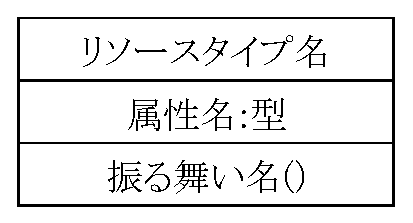
\includegraphics[scale=0.5]{img/resourceTypeSample.eps}
\caption{リソースタイプ}
\label{fig:resourceTypeSample}
\end{center}
\end{minipage}
\begin{minipage}{0.5\hsize}
\begin{center}

\includegraphics[scale=0.5]{img/resourceSample.eps}
\caption{リソース}
\label{fig:resourceSample}
\end{center}
\end{minipage}
\end{tabular}
\end{figure}

\begin{figure}[p]
\begin{tabular}{ccc}
\begin{minipage}{0.35\hsize}
\begin{center}
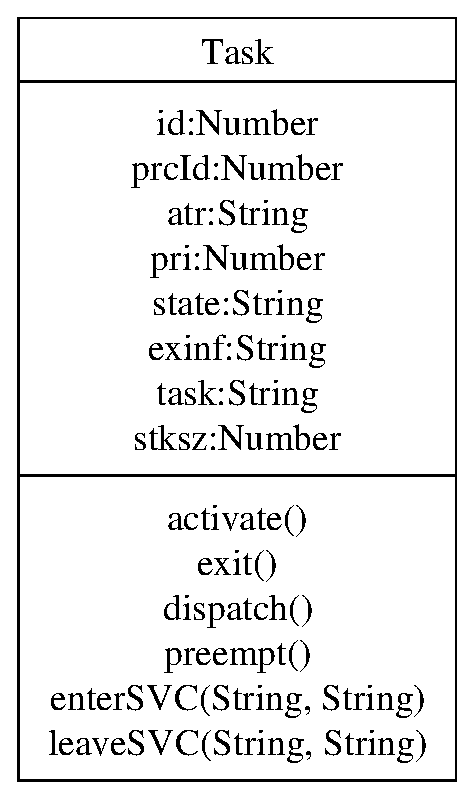
\includegraphics[scale=0.5]{img/resourceTypeSampleByTask.eps}
\caption{タスクをリソースタイプTaskとして表現した例}
\label{fig:resourceTypeSampleByTask}
\end{center}
\end{minipage}
\begin{minipage}{0.25\hsize}
\mbox{}\\
\end{minipage}
\begin{minipage}{0.3\hsize}
\begin{center}
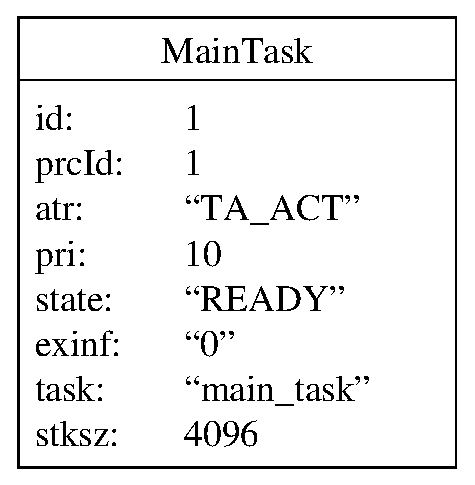
\includegraphics[scale=0.5]{img/resourceSampleByTask.eps}
\caption{リソースタイプTaskのリソースMainTaskの例}
\label{fig:resourceSampleByTask}
\end{center}
\end{minipage}
\end{tabular}
\end{figure}

\clearpage

\subsection{標準形式トレースログの定義}

本小節では,前小節で抽象化したトレースログを,標準形式トレースログとして形式化する.
標準形式トレースログの定義は,EBNF(Extended Backus Naur Form)および終端記号として正規表現を用いて行う.
正規表現はスラッシュ記号({\tt /})で挟むものとする.

前小節によれば,トレースログは,時系列にイベントを記録したものであるので,1つのログには時刻とイベントが含まれるべきである.
トレースログが記録されたファイルのデータを\verb|TraceLog|,\verb|TraceLog|を改行記号で区切った1行を\verb|TraceLogLine|とすると,これらは次のEBNFで表現される.

\begin{EBNF}
TraceLog = { TraceLogLine,"\n" };
TraceLogLine = "[",Time,"]",Event;
\end{EBNF}

\verb|TraceLogLine|は"\verb|[|","\verb|]|"で時刻を囲み,その後ろにイベントを記述するものとする.

時刻は\verb|Time|として定義され,次に示すように数値とアルファベットで構成するものとする.

\begin{EBNF}
Time = /[0-9a-Z]+/;
\end{EBNF}

アルファベットが含まれるのは,10進数以外の時刻を表現できるようにするためである.
これは,時刻の単位として「秒」以外のもの,たとえば「実行命令数」などを表現できるように考慮したためである.
この定義から,時刻には,2進数から36進数までを指定できることがわかる.

前小節にて,イベントを,リソースの属性の値の変化,リソースの振る舞いと抽象化した.
そのため,イベントを次のように定義した.

\begin{EBNF}
Event = Resource,".",(AttributeChange|BehaviorHappen);
\end{EBNF}

{\tt Resource}はリソースを表し,{\tt AttributeChange}は属性の値の変化イベント,{\tt BehaviorHappen}は振る舞いイベントを表す.
リソースはリソース名による直接指定,あるいはリソースタイプ名と属性条件による条件指定の2通りの指定方法を用意した.

リソースの定義を次に示す.

\begin{EBNF}
Resource = ResourceName
         | ResourceTypeName,"(",AttributeCondition,")";
ResourceName = Name;
ResourceTypeName = Name;
Name = /[0-9a-Z_]+/;
\end{EBNF}

リソースとリソースタイプの名前は数値とアルファベット,アンダーバーで構成されるとした.
{\tt AttributeCondition}は属性条件指定記述である.
これは次のように定義する.

\begin{EBNF}
AttributeCondition = BooleanExpression;
BooleanExpression = Boolean
   |ComparisonExpression
   |BooleanExpression,[{LogicalOpe,BooleanExpression}]
   |"(",BooleanExpression,")";
ComparisonExpression = AttributeName,ComparisonOpe,Value;
Boolean = "true"|"false";
LogicalOpe = "&&"|"||";
ComparisonOpe = "=="|"!="|"<"|">"|"<="|">=";
\end{EBNF}

属性条件指定は,論理式で表され,命題として属性の値の条件式を,等価演算子や比較演算子を用いて記述できるとした.

{\tt AttributeName}はリソース属性の名前であり,リソース名やリソースタイプ名と同様に,次のように定義する.

\begin{EBNF}
AttributeName = Name;
\end{EBNF}

イベントの定義にて,\verb|AttributeChange|は属性の値の変化を,\verb|BehaviorHappen|は振る舞いを表現しているとした.
これらは,リソースとドット"\verb|.|"でつなげることでそのリソース固有のものであることを示す.
リソースの属性の値の変化と振る舞いは次のように定義した.

\begin{EBNF}
AttributeChange = AttributeName,"=",Value;
Value = /[^"\\]+/;
BehaviorHappen =  BehaviorName,"(",Arguments,")";
BehaviorName = Name;
Arguments = [{Argument,[","]}];
Argument = /[^"\\]*/;
\end{EBNF}

属性の変化イベントは,属性名と変化後の値を代入演算子でつなぐことで記述し,振る舞いイベントは,振る舞い名に続けてカンマで区切った引数を括弧"{\tt ()}"で囲み記述するとした.


\subsection{標準形式トレースログの例}

前小節の定義を元に記述した,標準形式トレースログの例を表\ref{standartFormatTraceLogSample}に示す.

\begin{File}{標準形式トレースログの例}{standartFormatTraceLogSample}
[2403010]MAIN_TASK.leaveSVC(ena_tex,ercd=0)
[4496099]MAIN_TASK.state=READY
[4496802]TASK(state==RUNNING).state=READY
\end{File}

1行目がリソースの振る舞いイベントであり,2行目,3行目が属性の値の変化イベントである.
1行目の振る舞いイベントには引数が指定されている.

1行目,2行目はリソースを名前で直接指定しているが,3行目はリソースタイプと属性の条件によってリソースを特定している.


\section{標準形式への変換}

標準形式トレースログへの変換は,トレースログファイルを先頭から行単位で読み込み,変換ルールファイルで定義される置換ルールに従い標準形式トレースログに置換していくことで行われる.変換ルールファイルの詳細は\ref{subsec:cnvFile}小節で説明する.

1つの置換ルールに対して複数の標準形式トレースログを出力可能である.
しかし,所望の標準形式トレースログに変換する際,トレースログファイルの情報だけでは足りない場合がある.
例として,TOPPERS/ASPカーネル\cite{TOPPERS}というRTOSのトレースログを標準形式トレースログに変換することを考えてみる.
TOPPERS/ASPカーネルのトレースログの例を表\ref{aspLogSample}に示す.

\begin{File}{変換元となるTOPPERS/ASPカーネルのトレースログの例}{aspLogSample}
[1000]task 1 becomes RUNNABLE
[1005]dispatch to task 1.
[1100]task 1 becomes WAITING
\end{File}

表\ref{aspLogSample}のトレースログの内容を簡単に説明すると,時刻1000にタスクIDが1のタスクの状態がRUNNABLEになり,時刻1005に同タスクがディスパッチされ,時刻1100に同タスクの状態がWAITINGになったことを示している.
この場合,標準形式トレースログは表\ref{aspStandartLogSample}のように出力されることが要求される.
なお,説明のため簡略化しており,実際の変換結果とは異なる.

\begin{File}{表\ref{aspLogSample}を標準形式トレースログで表現した例}{aspStandartLogSample}
[1000]Task(id==1).activate()
[1000]Task(id==1).state = READY
[1005]Task(state==RUNNING).state=READY
[1005]Task(id==1).state = RUNNING
[1100]Task(id==1).state = WAITING
\end{File}

表\ref{aspLogSample}で示す元のトレースログが3行なのに対し,表\ref{aspStandartLogSample}で示す要求される標準形式トレースログは5行となっている.
これは,表\ref{aspStandartLogSample}の1行目と3行目が状況により追加されるからである.
表\ref{aspStandartLogSample}の1行目は,表\ref{aspLogSample}の1行目に対応しており,起動(\verb|activate()|)というタスクの振る舞いを可視化したいという要求があるため追加される必要がある.
また,表\ref{aspStandartLogSample}の3行目は,表\ref{aspLogSample}の2行目に対応しており,すでに起動しているタスクが横取りされて状態がREADYになる,という情報が元のトレースログに存在しないため,追加される必要がある.

しかしながら,これら標準形式トレースログの追加が必要になるのは一定の条件下のみである.
表\ref{aspStandartLogSample}の1行目は,タスクIDが1のタスクの状態が,時刻1000未満のときにDORMANTである場合だけである.
これは,起動という状態遷移を行うのが状態がDORMANTからREADYに遷移するときだけであり,状態がREADYになっただけでは起動であるのかどうか判断できないためである.
また,表\ref{aspStandartLogSample}の3行目が必要なときは,時刻1005のときに状態がRUNNINGのタスクが存在する場合だけである.

このように,リソース属性の遷移に伴うイベントや,元のトレースログに欠落している情報を補うイベントなど,元のトレースログの情報だけでは判断できないイベントを出力するには,特定時刻における特定リソースの有無やその数,特定リソースの属性の値などの条件で出力を制御できる必要がある.
そのため,TLVの変換ルールでは,置換する条件の指定と,条件指定の際に用いる情報を置換マクロを用いて取得できる仕組みを提供した.
具体的な記述例は\ref{subsec:cnvFile}小節で述べる.

標準形式トレースログに含まれるリソースは,リソースファイルで定義されていなければならない.
リソースファイルには,各リソースについて,その名前とリソースタイプ,必要であれば各属性の初期値を定義する.
リソースファイルの詳細については\ref{subsec:resFile}小節で述べる.
また,その際に使用されるリソースタイプはリソースヘッダファイルで定義されていなければならない.
リソースヘッダファイルには各リソースタイプについて,その名前と属性,振る舞いの定義を記述する.
リソースヘッダファイルの詳細については\ref{subsec:reshFile}小節で述べる.

リソースヘッダ,変換ルール,可視化ルールは可視化するターゲット毎に用意する.
その際のターゲットはリソースファイルに記述する.

\clearpage
\subsection{トレースログファイル}

標準形式トレースログに変換する元となるトレースログは,トレースログファイルとして読み込む.
トレースログファイルはテキストファイルであり,行単位でトレースログが記述されていなければならない.
これ以外のシンタックス,セマンティクスに関する制限はない.

任意のトレースログファイルを標準形式トレースログに変換するには,ターゲットとなるトレースログの形式毎に変換ルールファイルを用意する必要がある.

表\ref{aspTraceLog}に,RTOSであるTOPPERS/ASPカーネルのトレースログの例を示す.

\begin{File}{TOPPERS/ASPカーネルのトレースログの例}{aspTraceLog}
[11005239]: task 4 becomes RUNNABLE.
[11005778]: dispatch from task 2.
[11005954]: dispatch to task 4.
[11006160]: leave to dly_tsk ercd=0.
[11006347]: enter to dly_tsk dlytim=10.
[11006836]: task 4 becomes WAITING.
[11007050]: dispatch from task 4.
[11007226]: dispatch to task 2.
[11007758]: enter to sns_ctx.
[11007934]: leave to sns_ctx state=0.
[11008656]: enter to sns_ctx.
[11008832]: leave to sns_ctx state=0.
\end{File}

\subsection{リソースヘッダファイル}
\label{subsec:reshFile}

リソースヘッダファイルにはリソースタイプの定義を記述する.
リソースタイプの定義には,リソースタイプの名前,表示名,リソースタイプがもつ属性,振る舞いを記述する.

リソースヘッダは可視化するターゲット毎にリソースタイプを定義することができる.
つまり,タスクを表すリソースタイプ\verb|Task|を定義する際に,ターゲットとなるRTOS毎に属性の内容を変えたい場合,RTOS毎にリソースタイプ\verb|Task|を定義することができる.

表\ref{resourceHeaderSample}に,ターゲット\verb|asp|のリソースタイプ\verb|Task|を定義したリソースヘッダファイルの例を示す.
リソースヘッダファイルは,1つのオブジェクトで構成され,各メンバにターゲット毎のリソースタイプの定義を記述する.
メンバ名にターゲット名を記述し,値としてそのターゲットに属する複数のリソースタイプを定義したオブジェクトを記述する.
そのオブジェクトには,メンバ名にリソースタイプ名を,値にリソースタイプを定義したオブジェクトを記述する.
以下に,リソースタイプを定義するオブジェクトのメンバの説明と値について説明する.

\begin{File}{リソースヘッダファイルの例}{resourceHeaderSample}
{
  "asp":{
    "Task":{
      "DisplayName":"タスク",
      "Attributes":{
        "id":{
          "VariableType":"Number",
          "DisplayName":"ID",
          "AllocationType":"Static",
          "CanGrouping":false
        },
        "atr":{
          "VariableType":"String",
          "DisplayName":"属性",
          "AllocationType":"Static",
          "CanGrouping":false
        },
        /* 省略 */
        "state":{
          "VariableType":"String",
          "DisplayName":"状態",
          "AllocationType":"Dynamic",
          "CanGrouping":false,
          "Default":"DORMANT"
        }
      },
      "Behaviors":{
        "preempt":{"DisplayName":"プリエンプト"},
        "dispatch":{"DisplayName":"ディスパッチ"},
        "activate":{"DisplayName":"起動"},
        "exit":{"DisplayName":"終了"},
        /* 省略 */
        "enterSVC":{
          "DisplayName":"サービスコールに入る",
          "Arguments":{"name":"String","args":"String"}
        },
        "leaveSVC":{
          "DisplayName":"サービスコールから出る",
          "Arguments":{"name":"String","args":"String"}
        }
      }
    }
  }
}
\end{File}

\begin{description}
{\nopagebreak
\item[\texttt{DisplayName}] \mbox{}
    \begin{description}
    \setlength{\itemsep}{-1.5\itemsep}
    \item[説明] リソースタイプの表示名.主にGUI表示の際に用いられる
    \item[値] 文字列
    \end{description}
}
\clearpage
\item[\texttt{Attributes}] \mbox{}
    \begin{description}
    \setlength{\itemsep}{-1.5\itemsep}
    \item[説明] 属性の定義
    \item[値] オブジェクト.メンバ名に属性名,値に属性の定義をオブジェクトで記述する.その際のオブジェクトのメンバの説明は以下の通りである.
    
            \begin{description}
            \setlength{\itemsep}{-1.5\itemsep}
            {\nopagebreak
            \item[\texttt{VariableType}] \mbox{}
            \vspace{-0.25zw}
                \begin{description}
                \item[説明] 属性値の型
                \item[値] 文字列(\verb|"Number"|:数値,\verb|"Boolean"|:真偽値,\verb|"String"|:文字列のいずれか)
                \end{description}
            }{\nopagebreak
            \item[\texttt{DisplayName}] \mbox{}
            \vspace{-0.25zw}
                \begin{description}
                \item[説明] 属性の表示名.主にGUI表示の際に用いられる
                \item[値] 文字列
                \end{description}
            }{\nopagebreak
            \item[\texttt{AllocationType}] \mbox{}
            \vspace{-0.25zw}
                \begin{description}
                \item[説明] 属性の値が動的か静的かの指定.ここで動的とは,属性値変更イベントが発生すること指し,静的とは発生しないことを指す.
                \item[値] 文字列(\verb|"Static"|,\verb|"Dynamic"|のいずれか)
                \end{description}
            }{\nopagebreak
            \item[\texttt{CanGrouping}] \mbox{}
            \vspace{-0.25zw}
                \begin{description}
                \item[説明] リソースをグループ化できるかどうか.ここで\verb|true|を指定された場合,GUIでリソースの一覧を表示する際に初期値でグループ化され表示することができる.
                \item[値] 真偽値
                \end{description}
            }
            \end{description}
    \end{description}
\item[\texttt{Behaviors}] \mbox{}
    \begin{description}
    \setlength{\itemsep}{-1.5\itemsep}
    \item[説明] 振る舞いの定義
    \item[値] オブジェクト.メンバ名に振る舞い名,値に振る舞いの定義をオブジェクトで記述する.その際のオブジェクトのメンバの説明は以下の通りである.
    
            \begin{description}
            \setlength{\itemsep}{-1.5\itemsep}
            {\nopagebreak
            \item[\texttt{DisplayName}] \mbox{}
            \vspace{-0.25zw}
                \begin{description}
                \item[説明] 振る舞いの表示名.主にGUI表示の際に用いられる
                \item[値] 文字列
                \end{description}
            }{\nopagebreak
            \item[\texttt{Arguments}] \mbox{}
            \vspace{-0.25zw}
                \begin{description}
                \item[説明] 振る舞いの引数
                \item[値] オブジェクト.メンバ名に引数名,値に引数の型を記述する.
                \end{description}
            }
            \end{description}
    \end{description}
\end{description}

\clearpage
\subsection{リソースファイル}
\label{subsec:resFile}

リソースファイルには,主に,標準形式トレースログに登場するリソースの定義を記述する.
他にも,時間の単位や時間の基数,適用する変換ルール,リソースヘッダ,可視化ルールを定義する.
リソースの定義には,名前とリソースタイプ,必要があれば属性の初期値を記述する.

表\ref{resourceSample}にリソースファイルの例を示す.
リソースファイルは1つのオブジェクトで構成され,\verb|TimeScale|,\verb|TimeRadix|,\verb|ConvertRules|,\verb|VisualizeRules|,\verb|ResourceHeaders|,\verb|Resources|の6つのメンバを持つ.
以下にそれぞれのメンバについて説明する.

\begin{FileHere}{リソースファイルの例}{resourceSample}
{
  "TimeScale" :"us",
  "TimeRadix" :10,
  "ConvertRules"   :["asp"],
  "VisualizeRules" :["toppers","asp"],
  "ResourceHeaders":["asp"],
  "Resources":{
    "TASK1":{
      "Type":"Task",
      "Color":"ff0000",
      "Attributes":{
        "id"    :1,
        "atr"   :"TA_NULL",
        "pri"   :10,
        "exinf" :1,
        "task"  :"task",
        "stksz" :4096,
        "state" :"DORMANT"
      }
    },
    "TASK2":{
      "Type":"Task",
      "Color":"00ff00",
      "Attributes":{
        "id"    :4,
        "atr"   :"TA_ACT",
        "pri"   :5,
        "exinf" :0,
        "task"  :"task",
        "stksz" :4096,
        "state" :"READY"
      }
    }
  }
}
\end{FileHere}

\begin{description}
{\nopagebreak
\item[\texttt{TimeScale}] \mbox{}
    \begin{description}
    \setlength{\itemsep}{-1.5\itemsep}
    \item[説明] 時間の単位
    \item[値] 文字列
    \end{description}
}{\nopagebreak
\item[\texttt{TimeRadix}] \mbox{}
    \begin{description}
    \setlength{\itemsep}{-1.5\itemsep}
    \item[説明] 時間の基数
    \item[値] 数値
    \end{description}
}{\nopagebreak
\item[\texttt{ConvertRules}] \mbox{}
    \begin{description}
    \setlength{\itemsep}{-1.5\itemsep}
    \item[説明] 適用する変換ルールのターゲット.複数のターゲットを指定可能
    \item[値] 文字列の配列
    \end{description}
}
{\nopagebreak
\item[\texttt{VisualizeRules}] \mbox{}
    \begin{description}
    \setlength{\itemsep}{-1.5\itemsep}
    \item[説明] 適用する可視化ルール.複数のターゲットを指定可能
    \item[値] 文字列の配列
    \end{description}
}{\nopagebreak
\item[\texttt{ResourceHeaders}] \mbox{}
    \begin{description}
    \setlength{\itemsep}{-1.5\itemsep}
    \item[説明] \verb|Resources|で定義されるリソースのリソースタイプを定義しているターゲット.複数のターゲットを指定可能
    \item[値] 文字列の配列
    \end{description}
}
\item[\texttt{Resources}] \mbox{}
    \begin{description}
    \setlength{\itemsep}{-1.5\itemsep}
    \item[説明] リソースを定義
    \item[値] オブジェクト.メンバ名にリソースの名前,値にリソースの定義をオブジェクトで記述.値として与えるオブジェクトで使えるメンバは以下のとおりである.
    
        \begin{description}
        {\nopagebreak
        \item[\texttt{Type}]  \mbox{}
            \vspace{-0.25zw}
            \begin{description}
            \setlength{\itemsep}{-1.5\itemsep}
            \item[説明] 必須項目である.リソースタイプ名を記述
            \item[値] 文字列
            \end{description}
        }{\nopagebreak
        \item[\texttt{Color}]  \mbox{}
            \vspace{-0.25zw}
            \begin{description}
            \setlength{\itemsep}{-1.5\itemsep}
            \item[説明] リソース固有の色を指定.可視化表示の際に用いられる
            \item[値] 文字列.RGBを各8bitで表現したものを16進法表記で記述
            \end{description}
        }{\nopagebreak
        \item[\texttt{Attributes}]  \mbox{}
            \vspace{-0.25zw}
            \begin{description}
            \setlength{\itemsep}{-1.5\itemsep}
            \item[説明] 属性の初期値.指定できる属性はリソースタイプで定義されているものに限る
            \item[値] オブジェクト.メンバ名に属性名,値に属性の初期値を記述
            \end{description}
        }
        \end{description}
    \end{description}
\end{description}

\subsection{変換ルールファイル(JSON形式)}
\label{subsec:cnvFile}

変換ルールファイルには,ターゲットとなるトレースログを標準形式トレースログに変換するためのルールが記述される.
表\ref{convertRuleFileSample}に,変換ルールファイルの例を示す.

\begin{table}[h]
{\scriptsize
\begin{quote}
\bkcounttrue
\caption{変換ルールファイルの例}
\label{convertRuleFileSample}
\begin{breakbox}
\setlength{\baselineskip}{0.8\normalbaselineskip}
\begin{verbatim}
{
  "asp":{
    "\[(?<time>\d+)\] dispatch to task (?<id>\d+)\.":[
      {
        "$EXIST{[${time}]Task(state==RUNNING)}":[
          "[${time}]$RES_NAME{[${time}]Task(state==RUNNING)}.preempt()",
          "[${time}]$RES_NAME{[${time}]Task(state==RUNNING)}.state=READY"
        ]
      },
      "[${time}]$RES_NAME{Task(id==${id})}.dispatch()",
      "[${time}]$RES_NAME{Task(id==${id})}.state=RUNNING"
    ],
    "\[(?<time>\d+)\] task (?<id>\d+) becomes (?<state>[^\.]+)\.":[
      {
        "$ATTR{[${time}]Task(id==${id}).state}==DORMANT && ${state}==READY"
          :"[${time}]$RES_NAME{Task(id==${id})}.activate()",
        "$ATTR{[${time}]Task(id==${id}).state}==RUNNING && ${state}==DORMANT"
          :"[${time}]$RES_NAME{Task(id==${id})}.exit()",
      },
      "[${time}]$RES_NAME{Task(id==${id})}.state=${state}"
    ],
    "\[(?<time>\d+)\] enter to (?<name>\w+)( (?<args>.+))?\.?":{
      "$EXIST{[${time}]Task(state==RUNNING)}"
        :"[${time}][${time}]Task(state==RUNNING).enterSVC(${name},${args})"
    },
    "\[(?<time>\d+)\] leave to (?<name>\w+)( (?<args>.+))?\.?":{
      "$EXIST{[${time}]Task(state==RUNNING)}"
        :"[${time}][${time}]Task(state==RUNNING).leaveSVC(${name},${args})"
    }
  }
}
\end{verbatim}
\end{breakbox}
\end{quote}
}
\end{table}

変換ルールファイルは,1つのオブジェクトで構成され,各メンバにターゲット毎の変換ルールを記述する.
メンバ名にターゲット名を記述し,値としてそのターゲットが出力するトレースログを標準形式へ変換するためのルールをオブジェクトとして記述する.
そのオブジェクトのメンバ名には,標準形式へ変換される対象となるトレースログを正規表現を用いて記述し,値には出力する標準形式トレースログを記述する.
この際,値を文字列として記述すれば1行を,文字列の配列として記述すれば複数行を出力することができる.
また,値としてオブジェクトを記述することで,そのメンバ名に出力する条件を記述し,値に出力する標準形式トレースログを記述すれば,条件が真のときのみ出力するように定義できる.
また,このときの配列やオブジェクトはネストして記述することができる.

表\ref{convertRuleFileSample}の例を用いて具体的な説明を行う.
3行目,13行目,22行目,26行目が検索するトレースログの正規表現である.
これらの正規表現に一致するトレースログが見つかったとき,対応する値の標準形式トレースログが出力される.
3行目,13行目の正規表現に一致した場合は,標準形式トレースログが配列として与えられていて,複数の標準形式トレースログを出力する可能性がある.
3行目の正規表現に一致した場合は,10行目,11行目は必ず出力され,6行目,7行目の標準形式トレースログは5行目の条件が真の場合に出力される.
13行目の正規表現に一致した場合は,18行目は必ず出力され,16行目,18行目の標準形式トレースログはそれぞれ15行目,17行目の条件が真の場合に出力される.
22行目,26行目の正規表現に一致した場合は,標準形式トレースログがオブジェクトとして与えられていて,それぞれ23行目,27行目の条件が真の場合のみ標準形式トレースログを出力する.

検索するトレースログの正規表現において,名前付きグループ化構成体を用いると,入力文字列中の部分文字列をキャプチャすることができ,標準形式トレースログの出力や条件判定の際に使用できるようになる.名前付きグループ化構成体は"\texttt{(?<}\textit{name}\texttt{>}\textit{regexp}\texttt{)}"と記述する.このとき,\textit{regexp}で表現される正規表現にマッチする部分文字列が\textit{name}をキーとしてキャプチャされる.キャプチャされた文字列は,キーを用いて"\verb|${|\textit{name}\verb|}|"と記述することで呼び出せる.
また,名前付きでないグループ化構成体"\texttt{(}\textit{regexp}\texttt{)}"を用いることもでき,その際は"\texttt{\$}\textit{n}"で呼び出せる.\textit{regexp}に一致した部分文字列に1から順に番号がつけられ,これを呼び出す際の番号\textit{n}として用いる.

\subsubsection{置換マクロ}
標準形式トレースログをオブジェクトとして記述することで出力を条件で制御できることを上記で述べたが,条件判定の際に置換マクロを用いることで特定リソースの有無や数,属性の値を得ることができる.
また,置換マクロは,条件判定のときだけでなく,出力する標準形式トレースログの記述にも用いることができる.
置換マクロは"\verb|$|{\it name}\verb|{|{\it common-tracelog-syntax}\verb|}|"という形式で記述する.{\it name}は置換マクロ名であり,{\it common-tracelog-syntax}は標準形式トレースログの文字列である.{\it common-tracelog-syntax}にはリソースや属性が指定され,時刻の指定も可能である.
利用できる置換マクロは以下の通りである.

\vspace{1zw}
{\nopagebreak
\noindent
\verb|$EXIST{|\textit{resource}\verb|}|
\vspace{-0.75zw}
\begin{quote}
指定されたリソース{\it resource}が存在すれば{\tt true},存在しなければ{\tt false}に置換される.
リソースがリソース名ではなく,リソースタイプと属性の条件で記述されることを想定している.

\begin{description}
\item[例] 時刻1000に属性{\tt state}の値が{\tt RUNNING}であるリソースタイプ{\tt Task}のリソースが存在する場合

\hspace*{-1zw}入力\vspace{-1.75zw}
\begin{EBNF}
$EXIST{[1000]Task(state==RUNNING)}
\end{EBNF}
\hspace*{-1zw}出力\vspace{-1.75zw}
\begin{EBNF}
true
\end{EBNF}
\end{description}

\end{quote}
}
{\nopagebreak
\noindent
\verb|$COUNT{|\textit{resource}\verb|}|
\vspace{-0.75zw}
\begin{quote}
指定されたリソース{\it resource}の数に置換される.
リソースがリソース名ではなく,リソースタイプと属性の条件で記述されることを想定している.

\begin{description}
\item[例] 時刻1000に属性{\tt state}の値が{\tt WAITING}であるリソースタイプ{\tt Task}のリソースが3つ存在する場合

\hspace*{-1zw}入力\vspace{-1.75zw}
\begin{EBNF}
$COUNT{[1000]Task(state==WAITING)}
\end{EBNF}
\hspace*{-1zw}出力\vspace{-1.75zw}
\begin{EBNF}
3
\end{EBNF}
\end{description}

\end{quote}
}
{\nopagebreak
\noindent
\verb|$ATTR{|\textit{attribute}\verb|}|
\vspace{-0.75zw}
\begin{quote}
指定された属性{\it attribute}の値に置換される.
リソースをリソースタイプと属性の条件で記述する場合は,条件に一致するリソースが1つになるようにしなければならない.

\vspace{-1zw}
\begin{description}
\item[例] 時刻1000にリソース{\tt MAIN\_TASK}の属性{\tt state}の値が{\tt WAITING}である場合

\hspace*{-1zw}入力\vspace{-1.75zw}
\begin{EBNF}
$ATTR{[1000]MAIN_TASK.state}
\end{EBNF}
\hspace*{-1zw}出力\vspace{-1.75zw}
\begin{EBNF}
WAITING
\end{EBNF}
\end{description}

\end{quote}
}
{\nopagebreak
\noindent
\verb|$RES_NAME{|\textit{resource}\verb|}|
\vspace{-0.5zw}
\begin{quote}
指定されたリソース{\it resource}の名前に置換される.
リソースをリソースタイプと属性の条件で記述する場合は,条件に一致するリソースが1つになるようにしなければならない.

\begin{description}
\item[例] 属性{\tt id}の値が{\tt 1}であるリソースタイプ{\tt Task}のリソースの名前がMAIN\_TASKのとき

\hspace*{-1zw}入力\vspace{-1.75zw}
\begin{EBNF}
$RES_NAME{Task(id==1)}
\end{EBNF}
\hspace*{-1zw}出力\vspace{-1.75zw}
\begin{EBNF}
MAIN_TASK
\end{EBNF}
\end{description}

\end{quote}
}
{\nopagebreak
\noindent
\verb|$RES_DISPLAYNAME{|\textit{resource}\verb|}|
\vspace{-0.5zw}
\begin{quote}
指定されたリソース{\it resource}の表示名に置換される.
リソースの表示名はリソースファイルで定義される.
リソースをリソースタイプと属性の条件で記述する場合は,条件に一致するリソースが1つになるようにしなければならない.

\begin{description}
\item[例] 属性{\tt id}の値が{\tt 1}であるリソースタイプ{\tt Task}のリソースの表示名が"メインタスク"のとき

\hspace*{-1zw}入力\vspace{-1.75zw}
\begin{EBNF}
$RES_DISPLAYNAME{Task(id==1)}
\end{EBNF}
\hspace*{-1zw}出力\vspace{-1.75zw}
\begin{EBNF}
メインタスク
\end{EBNF}
\end{description}

\end{quote}
}
{\nopagebreak
\noindent
\verb|$RES_COLOR{|\textit{resource}\verb|}|
\vspace{-0.5zw}
\begin{quote}
指定されたリソース{\it resource}の色に置換される.
リソースの色はリソースファイルで定義される.
リソースをリソースタイプと属性の条件で記述する場合は,条件に一致するリソースが1つになるようにしなければならない.

\begin{description}
\item[例] 属性{\tt id}の値が{\tt 1}であるリソースタイプ{\tt Task}のリソースの色が赤(ff0000)のとき

\hspace*{-1zw}入力\vspace{-1.75zw}
\begin{EBNF}
$RES_COLOR{Task(id==1)}
\end{EBNF}
\hspace*{-1zw}出力\vspace{-1.75zw}
\begin{EBNF}
ff0000
\end{EBNF}
\end{description}

\end{quote}
}

\subsection{変換ルールファイル(外部プロセス形式)}
ターゲットとなるトレースログを標準形式トレースログに変換するため外部プロセスも用いることも可能である.
外部プロセスを指定する方法は,別途「スクリプト拡張マニュアル」において説明する.
